% !TeX spellcheck = en_US
\documentclass[french]{yLectureNote}

\title{Mécanique du solide}
\subtitle{Physique}
\author{Paulhenry Saux}
\date{\today}
\yLanguage{Français}

\professor{F.Pettinari}
\usepackage{graphicx}%----pour mettre des images
\usepackage[utf8]{inputenc}%---encodage
\usepackage{geometry}%---pour modifier les tailles et mettre a4paper
%\usepackage{awesomebox}%---pour les boites d'exercices, de pbq et de croquis ---d\'esactiv\'e pour les TP de PC
\usepackage{tikz}%---pour deiffner + d\'ependance de chemfig
% \usepackage{tabularx}%---pour dimensionner automatiquement les tableaux avec variable X
\usepackage{awesomebox}%---Pour les boites info, danger et autres
\usepackage{menukeys}%---Pour deiffner les touches de Calculatrice
\usepackage{fancyhdr}%---pour les en-t\^ete personnalis\'ees
\usepackage{blindtext}%---pour les liens
\usepackage{hyperref}%---pour les liens (\`a mettre en dernier)
\usepackage{caption}%---pour la francisation de la l\'egende table vers Tableau
\usepackage{pifont}
\usepackage{array}%---pour les tableaux
\usepackage{lipsum}
\usepackage{yFlatTable}

\usepackage{multicol}

\newcommand{\Lim}[1]{\lim\limits_{\substack{#1}}\:}
\renewcommand{\vec}{\overrightarrow}
\newcommand{\N}[0]{\mathbb{N}}
\newcommand{\dd}{\mathrm{d}}
\newcommand{\norm}[1]{||\vec{#1}||}
\newcommand{\fo}{\psi(\vec{r},t)}
\newcommand{\foe}{\psi(\vec{r},t)\*}
\newcommand{\HH}{\hat{H}}
\newcommand{\hb}{\hbar}
\newcommand{\lap}{\nabla^2}
\newcommand{\lapcc}{\frac{\partial^2 }{\partial x^2}+\frac{\partial^2 }{\partial y^2}+\frac{\partial^2 }{\partial z^2}}
\begin{document}
\setcounter{chapter}{1}
\chapter{Cinématique - Méthodologie}
\section{Centre de masse}
% On considère un solide qui correspond à uen distribution continue de points matériels. La masse est définie par \[M = \int\int\int \rho(A)\dd V\] si le solide est un volume avec A un point quelconque de S et \(\rho(A)\) une masse volumique autour de A.
\begin{definition}[Centre de masse ou centre d'inertie]
Noté C ou G, il est défini par \[M\vec{OC} = \int_{S} \vec{OA}\cdot \dd m = \int_V \vec{OA} \cdot \rho(A)\dd V\]
\end{definition}
\subsection{Exemples}
\subsubsection{Part de tarte}
On cherche le centre de masse d'une part de tarte d'angle \(2\alpha\) et de rayon \(R\). Avec les règles de symétrie, on obtient facilement\marginInfo{La part de tarte est placée de telle façon qu'il y a un axe de symétrie le long de l'axe x} que \(y_G = z_G = 0\). Trouvons maintenant \(x_G\) :
\explanation{t1}{On convertit le \(x\) en coordonnée polaires pour trouver \(\rho\cos(\varphi)\)}
\explanation{t2}{On sépare les intégrales}
\explanation{t3}{L'aire de la tarte dans son ensemble est \(\pi R^2\). Comme on prend un angle de \(2\alpha\), on prend la fraction qui coorespond à une moitié de tarte, soit \(\frac{2\alpha}{2\pi} = \alpha\) et \(S = \alpha R^2\)}
\begin{flalign*}
x_G &= \frac{1}{M} \int\int x \sigma \dd S\\
&= \frac{1}{S} \int\int \rho\cos(\varphi) \rho\dd \rho\dd \varphi\explain{t1}{left}{0}{0.5}{×}\\
&= \frac{1}{S}\int_0^R \rho^2\dd \rho \int_{-\alpha}^{\alpha}\cos(\varphi)\dd \varphi\explain{t2}{left}{0}{0.5}{×}\\
&= \frac{2R^3}{3S}\sin(\alpha)\\
&=\frac{2}{3}\frac{\sin(\alpha)}{\alpha}R\explain{t3}{left}{0}{0.5}{×}
\end{flalign*}
\subsubsection{Centre de masse d'un c\^one homogène}%polyco
% On considère un c\^one crux de densité surfacique \(\sigma\) et d'élément de surface \(\dd S\)
\includegraphics[scale=0.5]{methode-2}

On définit la hauteur du c\^one \(h\) et \(\alpha\) le demi angle du cone à partir du sommet. On sait par symétrie que le cdm se trouve sur l'axe perpendiculaire à la base et passant par le sommet. Reste à savoir où il se trouve sur l'axe \(Oz\).
On prend \(\dd S = \rho\dd \varphi\dd l\) avec \(\rho = z\tan(\alpha), l = \frac{z}{\cos(\alpha)}\), donc \(\dd l = \frac{\dd z}{\cos(\alpha)}\).
\begin{flalign*}
M\times z_G &= \int_{A} z\sigma \dd A\\
&= \int_{A} z\sigma \dd r\dd \theta \dd l\\
&= \int_{A} z\sigma z\tan(\alpha) \dd \theta \frac{\dd z}{\cos(\alpha)} \\
&= \sigma \frac{\tan(\alpha)}{\cos(\alpha)} \int_{A} z^2 \dd \theta \dd z \\
&= \sigma \frac{\tan(\alpha)}{\cos(\alpha)} \int_{0}^h z^2\dd z \int^{2\pi}_0 \dd \theta  \\
&= \sigma \frac{\tan(\alpha)}{\cos(\alpha)} \times \frac{h^3}{3} \times 2\pi  \\
\end{flalign*}
On calcule de la m\^eme façon M pour trouver \[M = \int_{(S)} \sigma \dd S = 2\pi \sigma \frac{\tan(\alpha)h^2}{2\cos(\alpha)}\]
On en déduit que, en injectant l'expression de M dans les calculs précédents :
\[z_G = \frac{2}{3}h\]


% \begin{flalign*}
% Mz_C = \int\int\int_S \dd m z
% \end{flalign*}


% Donc
% \begin{flalign*}
% M\cdot z_c &= \int\int\sigma \dd S\cdot z = \sigma \int_0^{2\pi}\int_0^{h}\rho\dd \varphi \dd l \cdot z\\
% &= \sigma\int_0^{2\pi}\dd \varphi\int_0^hz\frac{\rho}{h}\frac{\dd z}{\cos(\alpha)}\\
% &= \sigma 2\pi \frac{\rho}{h}\frac{1}{\cos(\alpha)}\frac{h^3}{3}\\
% M &= \int\int\sigma \dd S\\
% &= 2\pi\sigma \frac{\tan(\alpha)}{\cos(\alpha)}\frac{h^2}{2}\\
% z_c &= \frac{2}{3}h
% \end{flalign*}
\subsubsection{Associativité du centre de masse : Exemple du disque évidé}
Prenons ce disque :

\includegraphics[scale=0.2]{disque}

On cherche le barycentre. Par symétrie, on sait que \(y_G=z_G = 0\). Reste à trouver \(x_G\). On introduit donc \(M_1 = \sigma \pi R^2_1\) et \(M_2 = -\sigma \pi R^2_2\). En appliquant la formule, on obtient\[x_g = \frac{\sigma \pi R_1^2\times 0 - \sigma \pi R_2^2\times a}{\sigma \pi (R_1^2-R_2^2)} = -a\frac{R_2^2}{R_1^2-R_2^2}\]

\section{Moment d'inertie}
\subsection{Méthode de calcul (symétrie de révolution)}
% Cas du cercle : \(z = 0, x^2+y^2 = R^2, \dd  m \lambda \dd l =\lambda R \dd \varphi \).
% Donc \(2I_{ox} = I_{oz} = \int R^2 \lambda R \dd \varphi \dd R = \lambda R^2 2 \pi\) et \(M = \int \dd m = R\lambda 2\pi\), donc \(I_{oz} = MR^2\)\marginWarning{Résultat à savoir}.
%
% Cas du disque : On a toujours \(z=0, x^2+y^2 = r^2, \dd m = \sigma \dd S\). On a aussi \(I_{ox} = \int_{0}^{2\pi}\int_0^R r^2\sigma r\dd \varphi\dd r = \sigma 2\pi \frac{R^4}{4}\) avec \(M = \int \sigma \dd S = \sigma \pi R^2\), donc \(I_{oz} = 2I_{oy} = M\frac{R^2}{2}\).
\subsubsection{Disque}
\criticalInfo{Différence de méthode}{Les méthodes présentées ici peuvent paraitre différentes de celles vues en cours. En réalité, elles reviennent au m\^eme, mais celles présentées ici sont plus générales (et plus rigoureuses) et serviront également en Électromagnétisme 1}
% On considère le disque comme une somme d'anneaux concentriques de rayon \(r\) et d'appaisseur \(\dd r\).
%
% On calcule d'abord \(\dd m = \sigma \dd A = \sigma 2\pi r\dd r\). En effet, on considère l'aire d'un anneau infiniment petit, donc de coté inférieur \(2\pi r\), le tout multiplié par la largeur \(\dd r\).
%
% Le moment d'inertie élémentaire \(\dd I\) de chaque anneau est donné par la formule \(\dd I=r^2\dd m\). En remplaçant \dd m, on obtient : \(\dd I = 2\pi \sigma r^3\dd r\).
%
% On intègre sur tout le rayon : \(I = \int_0^R \dd I = 2\pi \sigma r^3\dd r = 2\pi \sigma [\frac{r^4}{4}]^R_0 = \frac{\pi \sigma R^4}{2}\)
%
% On sait que \(\sigma = \frac{M}{\pi R^2}\), donc on en déduit que \[I = \frac{MR^2}{2}\]
\explanation{m1}{On remplace \(\dd A\) par l'élément de surface élémentaire en coordonnées polaires}
\explanation{m2}{On remplace \(\sigma\) par \(\frac{M}{A}\) car par définition \(\sigma A = M\)}
\begin{flalign*}
I_{oz}&= \int_{(S)} \dd I\\
&= \int_{(S)} r^2 \dd m\\
&= \int_{(S)} r^2 \sigma \dd A\\
&= \int_{(S)} r^2 \sigma r\dd r\dd \theta\explain{m1}{right}{0}{0.5}{×}\\
&= \sigma \int_{0}^R r^3\dd r \int_0^{2\pi}\dd \theta\\
&= \sigma \int_{0}^R r^3\dd r 2\pi\\
&= \sigma [\frac{r^4}{4}]_{0}^R 2\pi\\
&= \sigma \frac{R^4}{4} 2\pi\\
&= \frac{M}{A} \frac{R^4}{2} \pi\explain{m2}{right}{0}{0.5}{×}\\
&= \frac{M}{\pi R^2} \frac{R^4}{2} \pi\\
&= \frac{MR^2}{2}\\
\end{flalign*}
\subsubsection{Cercle}
On calcule de la m\^eme façon\marginTips{Cette méthode fonctionne également et est plus simple.
\begin{flalign*}
I_{oz} &= \int r^2 \dd m\\
&= \int R^2 \dd m\\
&= R^2 \int \dd m\\
&= R^2M
\end{flalign*}}
\begin{flalign*}
I_{oz}&= \int_{(S)} \dd I\\
&= \int_{(S)} r^2 \dd m\\
&= \int_{(S)} r^2 \lambda \dd L\\
&= \int_{(S)} r^2 \lambda r \dd \theta\\
&= R^2 \lambda R \int_{0}^{2\pi} \dd \theta\\
&= R^3 \lambda 2\pi\\
&= R^3 2\pi \frac{M}{L}\\
&= R^3 2\pi \frac{M}{2\pi R}\\
&= R^2M\\
\end{flalign*}

et \[I_{ox} = \frac{MR^2}{2}\]
% Pour la sphère creuse : On la considère comme une somme d'anneaux de rayon \(r = R\sin(\theta)\) avec \(R\) le rayon maximal et \(\theta\) l'angle par rapport à l'axe vertical et d'eppaisseur \(\dd s = R\dd \theta\). Sa surface élémentaire est donc \(\dd A = 2\pi r \times R\dd \theta = 2\pi R\sin(\theta)R\dd \theta = 2\pi R^2\sin(\theta)\dd \theta\)
% \begin{flalign*}
% I &= \int_S \dd I\\
% &= \int_S r^2 \dd m\\
% &= \int_S r^2 \sigma \dd A\\
% &= \int_S r^2 \frac{M}{2}\sin(\theta)\dd \theta\\
% &= \int_S (R\sin(\theta))^2 (\frac{M}{2}\sin(\theta)\dd \theta)\\
% &= \int_0^{\pi} \frac{MR^2}{2}\sin(\theta)^3\\
% &= \frac{MR^2}{2}\times \frac{4}{3}\\
% &= \frac{2}{3}MR^2
% \end{flalign*}
\subsubsection{Cylindre creux}
Pour l'axe z, le résultat est identique à celui d'un cercle\marginInfo{En effet, d'un point de vue de la rotation autour de l'axe, la masse est répartie de la même manière : elle est entièrement concentrée à une distance R de l'axe de rotation.}.

Pouyr l'axe x, avec la base du cylindre en \(-h/2\)\marginCritical{On peut aussi le calculer avec la base en 0. On trouvera un autre résultat \(\frac{Mh^2}{3}\), ce qui est logique, car il y aura plus de résistance en le faisant tourner autour de cet axe.}.
\begin{flalign*}
I_{ox} = I_{oy} = \frac12 I_{oz} &+ \int z^2\dd m\\
&+ \int z^2\sigma R\dd \varphi \dd z\\
&+ \sigma R \int_{0}^{2\pi}\dd \varphi\int_{-h/2}^{h/2} z^2\dd z\\
&+ \sigma R2\pi \frac{h^3}{12}\\
= \frac{MR^2}{2} &+ \frac{Mh^2}{12}
\end{flalign*}

% Pouyr l'axe x, avec la base du cylindre en 0, on obtient \[I_{ox} = \frac{MR^2}{2} + \frac{Mh^2}{12}\]

Si on considère un fil vertical, on obtiendra aussi \[I_{ox} = \frac{Mh^2}{12}\]

\subsubsection{Cylindre plein}
Le résultat est le m\^eme que pour le disque pour les m\^emes raisons.

\subsection{Méthode de calcul (symétrie sphérique)}
On aura toujours \(I_{oz} = I_{ox} = I_{oy}\)

On en déduit
\begin{flalign*}
3 I_{ox} &= 2(x^2+y^2+z^2)\dd m\\
&= 2\int r^2 \dd m = 2 I_o\\
&= \frac23 \int r^2 \dd m\\
\end{flalign*}
\subsubsection{Sphère creuse (Coque)}
On applique les m\^emes méthodes que précédenement, avec des coordonnées polaires et l'élément de surface élémentaire \(R\sin(\theta)\dd \theta \dd \varphi\), puis on multiplie le résultat par \(\frac23\) en raison de la propriété précédente.
\[I_o = \frac23 MR^2\]

\subsubsection{Sphère pleine}
\criticalInfo{Erreur courante}{Le calcul suivant de fonctionne pas
\begin{flalign*}
I_{oz}&= \int_{(S)} \dd I\\
&= \int_{(S)} r^2 \dd m\\
&= \int_{(S)} r^2 \sigma \dd V\\
&= \int_{(S)} r^2 \sigma r^2\sin(\theta)\dd r\dd \theta \dd \varphi\\
&= \sigma \int_{0}^R r^4\dd r \int_0^{2\pi}\dd \varphi \int_0^{\pi}\sin(\theta)\dd \theta\\
&= \sigma \frac{R^5}{5} \times 2\pi \times 2\pi\\
&= \sigma 4\pi \frac{R^5}{5}\\
\end{flalign*}
\begin{flalign*}
&= \frac{M}{V} 4\pi \frac{R^5}{5}\\
&= \frac{3M}{4\pi R^3} 4\pi \frac{R^5}{5} \pi\\
&= \frac{3MR^2}{5}\\
\end{flalign*}
Bien qu'il semble logique, on calcul ici, la distance par rapport au centre du cercle et non par rapport à un axe ! Il faut donc bien différencier les deux !
}
\explanation{m4}{Pour rappel, pour intégrer \(\sin^3\), on peut le remplacer par \((1-\cos^2)\sin\) et poser \(u = \cos(x)\)}
\begin{flalign*}
I_{oz}&= \int_{(S)} \dd I\\
&= \int_{(S)} r_a^2 \dd m\\
&= \int_{(S)} r_a^2 \sigma \dd V\\
&= \int_{(S)} r^2\sin(\theta)^2 \sigma r^2\sin(\theta)\dd r\dd \theta \dd \varphi\\
&= \int_{(S)} r^4 \sigma r^2\sin(\theta)^3\dd r\dd \theta \dd \varphi\\
&= \sigma \int_{0}^R r^4\dd r \int_0^{2\pi}\dd \varphi \int_0^{\pi}\sin(\theta)^3\dd \theta\\
&= \sigma \frac{R^5}{5} \times 2\pi \times \frac{4}{3}\explain{m4}{right}{0}{0.5}{×}\\
&= \sigma \frac{8}{3}\pi \frac{R^5}{5}\\
&= \frac{M}{V} \pi \frac{8 R^5}{15}\\
&= \frac{3M}{4\pi R^3} \pi \frac{8R^5}{15} \pi\\
&= \frac{2MR^2}{5}\\
\end{flalign*}
\[I_{ox} = \frac25 MR^2\]
% \section{Moment cinétique}
% \subsubsection{Solide avec point fixe O lié au solide}
% \explanation{d1}{A vérifie le théorème de Varignon}
% \explanation{d2}{On sait que \(\vec{a}\wedge (\vec{b}\wedge \vec{c}) = (\vec{a}\cdot \vec{c})\vec{b}-(\vec{b}\cdot\vec{a})\vec{c}\)}
% \begin{flalign*}
% \vec{L_{O/R}} = \int_{(S)} \vec{OA}\wedge \dd m \vec{v_{A\in S}}\\
% \end{flalign*}
% Avec O pt fixe du solide, A quelconque
% Mais A vérifie le théorème de Varignon, donc
% \[\vec{v_{A\in S/R}} = \vec{v_{O\in S/R}} + \vec{AO}\wedge \vec{\Omega} = \vec{AO}\wedge \vec{\Omega}\]
%
% On cherche \(\vec{OA}\wedge (\vec{OA}\wedge \vec{\Omega}) = \vec{OA}^2\cdot\vec{\Omega}-(\vec{OA}\cdot\vec{\Omega})\vec{OA}\)
%
% Donc \(\vec{L_{O/R}} = \int_{(S)} \vec{OA}^2\cdot\vec{\Omega}\dd m - \int_{(S)}(\vec{OA}\cdot\vec{\Omega})\vec{OA}\)
%
% En projetant \(\vec{L_{O/R}}\) sur les becteurs de la base de R, on obtient :
% \begin{flalign*}
% \vec{L_O}\cdot \vec{e_x} &= \int_{(S)} (x^2+y^2+z^2)\dd m \vec{\Omega} - \int (x\omega_x+y\omega_y+z\omega_z)\dd m\\
% &= \int_{(S)} (y^2+z^2)\dd m \omega_x - \int_{(S)} (yx\omega_y+zx\omega_z)\dd m\\
% &= I_{Ox}\omega_x - (I_{xy}\omega_y+I_{xz}\omega_z)\
% \end{flalign*}
%  De m\^eme, on aura \[L_{oy} = I_{Oy}\Omega_y - (I_{xy}\Omega_x+I_{zy}\Omega_z)\] et
%  \[L_{oz} = I_{Oz}\omega_z - (I_{xz\Omega_x+I_{zy}\Omega_z})\]
%
% On aura très souvent \(\vec{\omega}_S\) porté par un API donc \(\vec{L_{O/R}} = I_{O\Delta}\omega \vec{e_{\Delta}}\)
% \subsubsection{Cas général}
% Si il n'y a pas de point fixe lié au solide, on utilise le théorème de Koeing ou de transport du mouvement.
% \subsubsection{Exemple}
% On écrit \(\vec{\Omega_{OA}} = \dot{\theta_1}\vec{e_z}, \vec{\Omega_{OB}} = \dot{\theta_2}\vec{e_z} = (\dot{\theta_1}+\dot{\beta})\vec{e_z}\).
%
% Dans le solide \(OA\), O est fixe, donc on a \(\vec{L_{O/R}} = [I]_O \vec{\Omega_{OA/R}} = I_{oz}\dot{\theta_1}\vec{e_z}\) car OZ est un API.
%
% Dans \(AB\), pas de point fixe, donc \(\vec{L_{O/R}}(AB) = \vec{L*}(AB)+\vec{OC_2}\wedge \vec{V_C2/R}\) avec C2 le centre de masse de AB et M2 sa masse.
%
% On obtient \(\vec{L*}(AB) = \vec{L_{C2}}(AB) = I_{C2z}\dot{\theta_2}\vec{e_z}\) car \(C_2Z\) est un API.
%
% On obtient \(\vec{L_{O}}(OA+AB) = \vec{L_{O}(AO) + L_{O}(AB)}\)
\subsection{Astuce}
Dans le cas d'un disque pour avoir les moments par rapport aux axes, on fait \(I_{ox} + I_{oy}\) car \[I_{ox} = \iint (y^2+z^2)\sigma \dd S = \iint r^2\sin^2(\varphi)\sigma r\dd r \dd \varphi\] et
\[I_{oy} = \iint (x^2+z^2)\sigma \dd S = \iint r^2\cos^2(\varphi)\sigma r\dd r \dd \varphi\]

Comme ce n'est pas facile\marginCritical{Cela permet d'éviter de devoir linéariser des fonctions trigonométriques.}, on somme les 2 pour avoir l'identité \(\cos^2+\sin^2 = 1\) et on divise par 2 pour trouver \(I_{ox}\) ou \(I_{oy}\) car les 2 axes sont intergengeables.

Dans le cas d'une boule, c'est pareil : On peut addtionner les 3 moments d'inertie et obtenir :

\[3I_{ox} = I_O = I_{ox} + I_{oy} + I_{oz} = 2 \iiint r^2\dd m\] et \[I_O = \iiint_{(V)} r^2 \rho \dd V =\iiint_{(V)} r^4 \sin(\theta)\dd \theta \dd \varphi \dd r  = \frac{R^5}{5}\times 2\pi \times 2 = 4\pi \frac{R^5}{5} =  \frac{3}{5}R^2 \]

Il n'y a plus qu'à multiplier par \(\frac23\) pour trouver le résultat final :
\[I_{ox} = \frac{2}{5}R^2M\]
\section{Moment cinétique d'un solide en rotation}
\subsection{Cas d'un solide avec un point fixe O}

Considérons un solide (S) en rotation autour d'un point O qui est fixe dans le référentiel R. Le moment cinétique de ce solide par rapport à O est donné par la formule intégrale suivante :
$$
\vec{L}_{O/R} = \int_{(S)} \vec{OA} \wedge d\vec{p} = \int_{(S)} \vec{OA} \wedge \vec{v}_{A \in S/R} \, \dd m
$$
où $\vec{OA}$ est le vecteur position d'un point A du solide par rapport à O, et $\vec{v}_{A \in S/R}$ est la vitesse de ce point dans le référentiel R.

Puisque le point O est fixe dans R, la vitesse de tout point A du solide peut être exprimée en utilisant la formule de Varignon :
$$
\vec{v}_{A \in S/R} = \vec{v}_{O \in S/R} + \vec{\Omega} \wedge \vec{OA} = \vec{\Omega} \wedge \vec{OA}
$$
où $\vec{\Omega}$ est le vecteur de vitesse de rotation du solide.

En remplaçant cette expression dans la formule du moment cinétique :
$$
\vec{L}_{O/R} = \int_{(S)} \vec{OA} \wedge (\vec{\Omega} \wedge \vec{OA}) \, \dd m
$$
Avec
\begin{theorem}[Identité du double produit vectioriel]
\[\vec{a} \wedge (\vec{b} \wedge \vec{c}) = (\vec{a} \cdot \vec{c})\vec{b} - (\vec{a} \cdot \vec{b})\vec{c}\] avec \(\vec{a} = \vec{OA}\), \(\vec{b} = \vec{\Omega}\) et \(\vec{c} = \vec{OA}\)
\end{theorem}
l'intégrale devient :
$$
\vec{L}_{O/R} = \int_{(S)} \left( (\vec{OA} \cdot \vec{OA})\vec{\Omega} - (\vec{OA} \cdot \vec{\Omega})\vec{OA} \right) \, \dd m
$$
Soit\marginTips{Cette dernière équation est la relation générale entre le moment cinétique et la vitesse de rotation pour un solide avec un point fixe.} :
$$
\vec{L}_{O/R} = \left( \int_{(S)} OA^2 \, \dd m \right) \vec{\Omega} - \int_{(S)} (\vec{OA} \cdot \vec{\Omega})\vec{OA} \, \dd m
$$

Pour obtenir une expression plus explicite, nous projetons $\vec{L}_{O/R}$ sur les axes d'un repère orthonormé lié au solide
% (O, $\vec{e_x}$, $\vec{e_y}$, $\vec{e_z}$).
% Avec $\vec{OA} = x\vec{e_x} + y\vec{e_y} + z\vec{e_z}$ et $\vec{\Omega} = \omega_x\vec{e_x} + \omega_y\vec{e_y} + \omega_z\vec{e_z}$, la composante $L_{Ox}$ est
:
\begin{align*}
L_{Ox} &= \vec{L}_{O/R} \cdot \vec{e_x} \\
&= \int_{(S)} \left[ (x^2+y^2+z^2)\vec{\Omega} - (x\omega_x + y\omega_y + z\omega_z)(x\vec{e_x} + y\vec{e_y} + z\vec{e_z}) \right] \cdot \vec{e_x} \, \dd m \\
&= \int_{(S)} \left[ (x^2+y^2+z^2)\omega_x - (x\omega_x + y\omega_y + z\omega_z)x \right] \, \dd m \\
&= \int_{(S)} (x^2+y^2+z^2)\omega_x \, \dd m - \int_{(S)} (x^2\omega_x + xy\omega_y + xz\omega_z) \, \dd m \\
&= \int_{(S)} (y^2+z^2)\omega_x \, \dd m - \int_{(S)} (xy\omega_y + xz\omega_z) \, \dd m \\
&= \omega_x \int_{(S)} (y^2+z^2) \, \dd m - \omega_y \int_{(S)} xy \, \dd m - \omega_z \int_{(S)} xz \, \dd m
\end{align*}
En utilisant les définitions des moments et produits d'inertie :
\begin{itemize}
    \item $I_{Ox} = \int_{(S)} (y^2+z^2) \, \dd m$ (Moment d'inertie par rapport à l'axe Ox)
    \item $I_{xy} = \int_{(S)} xy \, \dd m$ (Produit d'inertie)
    \item $I_{xz} = \int_{(S)} xz \, \dd m$ (Produit d'inertie)
\end{itemize}
On obtient :
$$
L_{Ox} = I_{Ox}\omega_x - I_{xy}\omega_y - I_{xz}\omega_z
$$
De même, les autres composantes sont :
\begin{align*}
L_{Oy} &= -I_{yx}\omega_x + I_{Oy}\omega_y - I_{yz}\omega_z \\
L_{Oz} &= -I_{zx}\omega_x - I_{zy}\omega_y + I_{Oz}\omega_z
\end{align*}
En notation matricielle, ceci s'écrit $\vec{L}_O = [I]_O \vec{\Omega}$, où $[I]_O$ est la matrice d'inertie du solide au point O.

\subsection{Cas général : Théorème de transport (ou de Koenig)}

Si le solide n'a pas de point fixe, le moment cinétique par rapport à un point O (non lié au solide) est donné par le théorème de transport du moment cinétique\marginInfo{où C est le centre de masse du solide, $\vec{L}_{C/R}$ est le moment cinétique par rapport au centre de masse (moment cinétique propre), et $\vec{p}_{S/R} = M\vec{v}_{C/R}$ est la quantité de mouvement totale du solide de masse M.} :
$$
\vec{L}_{O/R} = \vec{L}_{C/R} + \vec{OC} \wedge \vec{p}_{S/R}
$$

Le moment cinétique propre $\vec{L}_{C/R}$ est calculé comme dans le cas du point fixe, mais en remplaçant O par C :
$$
\vec{L}_{C/R} = [I]_C \vec{\Omega}
$$

\subsection{Exemple d'application}

Considérons un système de deux solides, OA et AB, en mouvement.
\begin{itemize}
    \item Solide OA : O est un point fixe. L'axe de rotation est l'axe z. On a $\vec{\Omega}_{OA} = \dot{\theta_1}\vec{e_z}$. Si l'axe z est un axe principal d'inertie (API) pour le solide OA, alors les produits d'inertie correspondants sont nuls. Le moment cinétique est donc :
    $$
    \vec{L}_{O}(OA) = I_{Oz}\dot{\theta_1}\vec{e_z}
    $$
    \item Solide AB : Il n'a pas de point fixe. On utilise le théorème de Koenig. Le centre de masse est $C_2$. Le moment cinétique par rapport à O est :
    $$
    \vec{L}_{O}(AB) = \vec{L}_{C_2}(AB) + \vec{OC_2} \wedge M_2\vec{v}_{C_2/R}
    $$
    Le moment cinétique propre $\vec{L}_{C_2}(AB)$ est calculé par rapport à $C_2$. Si $C_2Z$ est un API pour le solide AB, alors :
    $$
    \vec{L}_{C_2}(AB) = I_{C_2z}\dot{\theta_2}\vec{e_z}
    $$
\end{itemize}
Le moment cinétique total du système par rapport à O est la somme des moments cinétiques de chaque solide :
$$
\vec{L}_{O}(OA+AB) = \vec{L}_{O}(OA) + \vec{L}_{O}(AB)
$$
 \end{document}
